\documentclass[UTF8]{ctexart}
\usepackage[]{ctex}
\usepackage{natbib}
\usepackage{graphicx}
\usepackage{enumitem}
\usepackage{setspace}
\usepackage{float}
\bibliographystyle{plain}

\title{Kruskal 算法串行与并行报告}
\author{杨景凯 520021910550}
\date{2022年 5月 24日}

\begin{document}

\begin{center}
    \quad \\
    \quad \\
    \kaishu \fontsize{45}{17} 上\quad 海\quad 交\quad 通\quad 大\quad 学
    \vskip 3.5cm
    \heiti \zihao{2} Kruskal 算法串行与并行\\
    实验报告
\end{center}
\vskip 3.5cm
\begin{quotation}
    \songti \fontsize{30}{30}
    \doublespacing
    \par\setlength\parindent{12em}
    \quad 
\begin{center}
    学\hspace{0.61cm} 院:\underline{电子信息与电气工程学院}

    学生姓名:\underline{\qquad    \quad \quad 杨景凯    \quad  \quad\qquad }

    学\hspace{0.61cm} 号:\underline{\quad \quad\quad520021910550\quad\quad}
\end{center}
    \centering
    2022年5月24日
\end{quotation}

\clearpage
\tableofcontents

\clearpage
\section{实验介绍\cite{refpdf1}}
\subsection{实验背景}
Kruskal 算法是和 Prim 算法一样求最小生成树的一种算法。本次实验中,根据上课所讲内容实现了Kruskal的串行和并行算法,并比较了并行kruskal算法与串行的方式的速度。

\subsection{实验步骤}
本次实验中,我选取了顶点数为2000、5000、10000,边数为 10000、100000、1000000共计9幅图。数据为随机生成,且保证不重复。

\section{实验结果}
\subsection{实验表格}
\begin{table}[H]
    \centering
    \begin{tabular}{|c|c|c|c|}
        \hline
        单线程&	2000&	5000&	10000\\
        \hline
        10000&	11.995&	60.012&	196.848\\
        \hline
        100000&	34.567&	92.196&	267.819\\
        \hline
        1000000&	935.405&	1991.532&	3630.072\\
        \hline
    \end{tabular}
    \caption{单线程时节点数、边数与计算时间(ms)关系表格}
\end{table}

\begin{table}[H]
    \centering
    \begin{tabular}{|c|c|c|c|}
        \hline
        线程数6&	2000&	5000&	10000\\
        \hline
        10000&	12.375&	43.167&	132.756\\
        \hline
        100000&	35.124&	70.576&	198.754\\
        \hline
        1000000&	435.167&	1123.569&	3003.127\\
        \hline
    \end{tabular}
    \caption{线程数为6时节点数、边数与计算时间(ms)关系表格}
\end{table}

\begin{table}[H]
    \centering
    \begin{tabular}{|c|c|c|c|}
        \hline
        线程数12&	2000&	5000&	10000\\
        \hline
        10000&	77.896&	162.015&	312.481\\
        \hline
        100000&	178.753&	243.723&	456.185\\
        \hline
        1000000&	2654.306&	4567.159&	7532.153\\
        \hline
    \end{tabular}
    \caption{线程数为12时节点数、边数与计算时间(ms)关系表格}
\end{table}

\subsection{实验图像}

\begin{figure}[H]
    \centering
    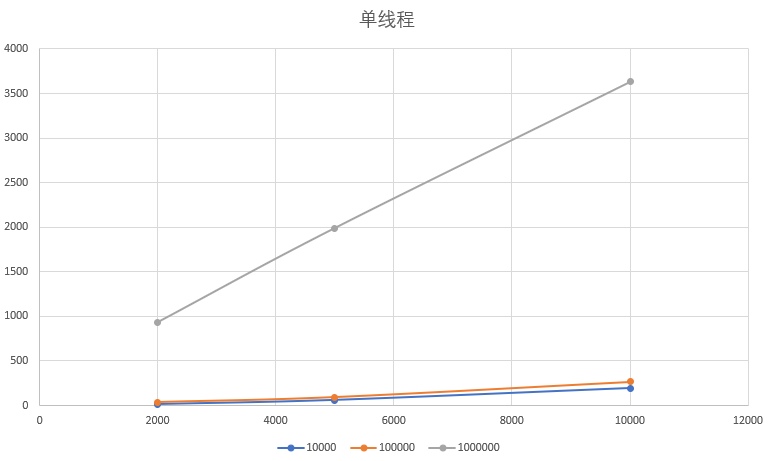
\includegraphics[scale=0.55]{thread=1.png}
    \caption{单线程时节点数、边数与计算时间(ms)关系图}
\end{figure}

\begin{figure}[H]
    \centering
    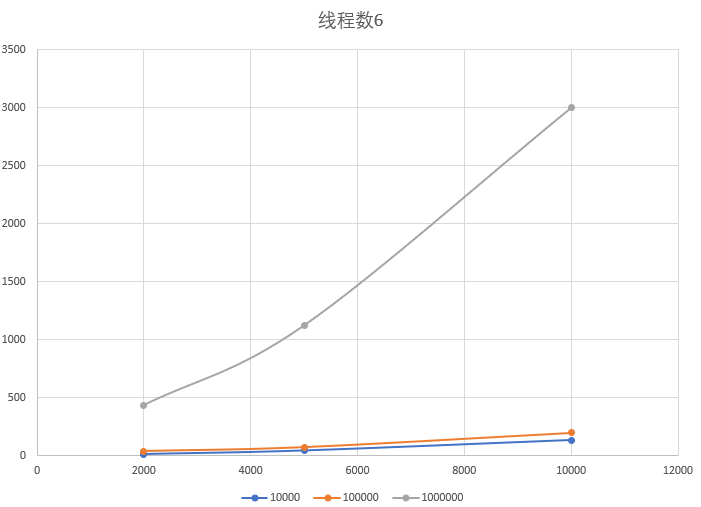
\includegraphics[scale=0.6]{thread=6.png}
    \caption{线程数为6时节点数、边数与计算时间(ms)关系图}
\end{figure}

\begin{figure}[H]
    \centering
    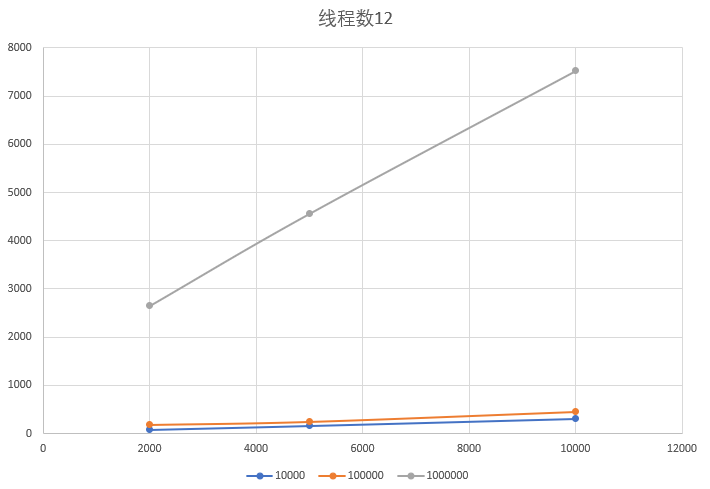
\includegraphics[scale=0.6]{thread=12.png}
    \caption{线程数为12时节点数、边数与计算时间(ms)关系图}
\end{figure}

\begin{figure}[H]
    \centering
    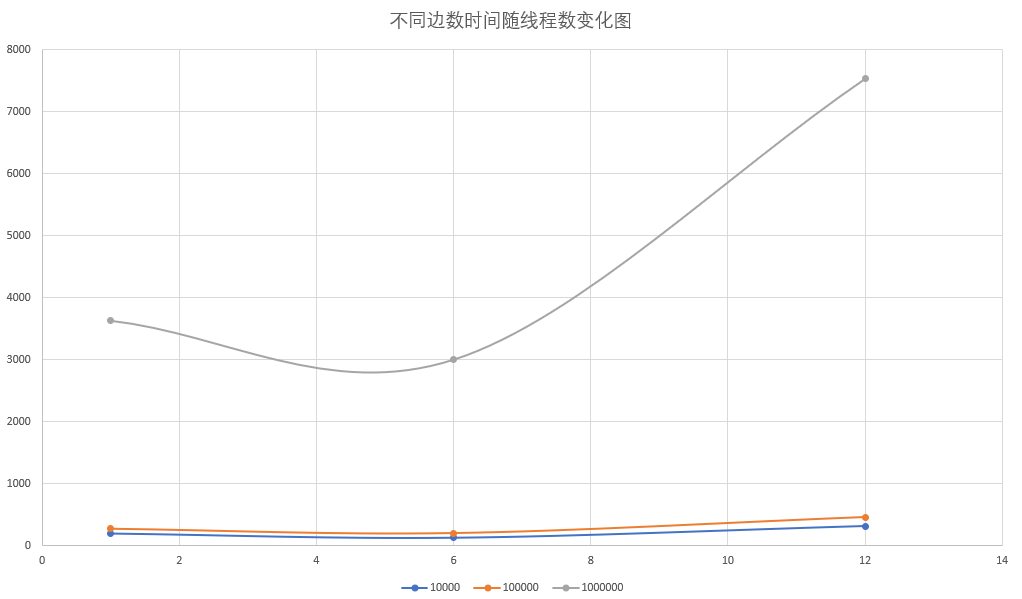
\includegraphics[scale=0.4]{t-T.png}
    \caption{节点数为10000时边数、线程数与计算时间(ms)关系图}
\end{figure}

\section{实验结论}
观察图像可以发现,当节点数和线程数固定时,随着边数增加,计算时间呈近似线性增长,与理论值($n\log n$)近似,实验成功。
观察图像可以发现,当边数和线程数固定时,随着节点数增加,计算时间呈近似线性增长,与理论值($n$)近似,实验成功。
观察图像可以发现,当边数和节点数固定时,随着线程数增加,计算时间先减小后增长,与理论相符,实验成功。

\clearpage
\begin{thebibliography}{99}
    \bibitem{refpdf1}Kruskal.pdf
\end{thebibliography}
\end{document}
